\documentclass[11pt,a4paper]{article}  % Déclare la classe du document.

\newcommand{\chaptermark}[2]{\og #2 \fg{} (#1)} % ligne uniquement pour éviter une erreur en cas d'article
\usepackage[table,dvipsnames,svgnames]{xcolor}
\usepackage{listingsutf8}
%\usepackage[utf8]{inputenc}% gestion des accents (source)
\usepackage[T1]{fontenc}% gestion des accents (PDF)
\usepackage{fontspec}
\usepackage[french]{babel}% gestion du français
\usepackage{textcomp}% caractères additionnels
\usepackage{mathtools,amssymb,amsthm}% packages de l'AMS + mathtools
\usepackage{amsmath}
\usepackage{yhmath}
\usepackage{mathpazo}
\usepackage[scaled=0.95]{helvet}
\usepackage{courier}
%\usepackage{fourier}
%\usepackage[scaled=0.95]{helvet}
%\usepackage{courier}
\usepackage{bm}
\usepackage{gensymb}
\usepackage{graphicx}

\usepackage{enumitem}
\usepackage{pifont}

\usepackage{pstricks}
\usepackage{pstricks-add}
\usepackage{pst-eucl}
\usepackage{pgfplots}
\let\clipbox\relax
%\usepackage{pst-plot,pst-text,pst-tree,pstricks-add}
%\usepackage{pst-node} % required package
\usepackage{pst-all}
\usepackage[most,skins,breakable]{tcolorbox}

\usepackage{euscript}





% ############### Nouvelles commandes ###############
% Coloration des labels des points dans pst-eucl
\makeatletter
\define@key[psset]{pst-eucl}{LabelColor}{\def\psk@LabelColor{#1}}
\psset{LabelColor=black}
\def\Pst@WhichLabel#1{{\color{\psk@LabelColor}%
		\ifx\psk@PointName\@default#1\else\psk@PointName\fi}}
\makeatother

% renomme le symbole #2 en #1#2 et invalide le symbole initial #2:
\def\renamesymbol#1#2{
	\expandafter\let\expandafter\newsym\expandafter=\csname#2\endcsname
	\expandafter\global\expandafter\let\csname#1#2\endcsname=\newsym
	\expandafter\global\expandafter\let\csname#2\endcsname=\origsym
}



\usepackage{ProfCollege}
\renamesymbol{Casio}{Calculatrice}
\usepackage[nonshellescape]{ProfLycee}



%\usepackage[left=1.5cm,right=1.5cm,top=2.5cm,bottom=2.5cm]{geometry}
\usepackage[left=13mm,right=13mm,top=18mm,bottom=18mm,footskip=30pt]{geometry}
\setlength{\headheight}{15pt}

\usepackage{titlesec}
\usepackage{pas-math}
\usepackage{longtable}
\usepackage{tikz,tkz-tab}
\usepackage{amsmath}
\usepackage[right]{eurosym}
\usepackage{sectsty}
\usepackage{tipfr}
\usepackage{setspace}

%pour faire les touches de la calculatrices
\usepackage{menukeys}
\renewmenumacro{\menu}{roundedmenus} % default: menus
\renewmenumacro{\directory}{pathswithfolder} % default: paths
\renewmenumacro{\keys}{shadowedroundedkeys} % default: roundedkeys


\usepackage{multicol}
\usepackage{multirow}
\usepackage{systeme}

%% Format des titres de chapitres, paragraphes, ...
\titleformat{\chapter}[frame]
{\color{red!85!white}\normalsize}%
{\filright\sffamily\Large%
	\enspace Chapitre \thechapter\enspace}%
{8pt}
{\color{red!85!white}\rule{0pt}{30pt}\sffamily\Huge\bfseries\filcenter}
%%%%%%%%%%%%%%%%%%%%
\titlespacing{\chapter}{0pc}{0pc}{2pc}
\titlespacing{\subsection}{2pc}{}{}

\titleformat{\subsection}[block]{\hspace{1em}}{\thesubsection}{1em .}{}
\titleformat{\subsubsection}[block]{\hspace{2em}}{\thesubsection}{1em )}{}

\chapterfont{\color{red}{}}
\sectionfont{\color{green!55!black}{}}
\subsectionfont{\color{cyan!65!black}{}}
\subsubsectionfont{\color{violet}{}}
\renewcommand{\thesection}{\color{green!55!black}\Roman{section}.}
\renewcommand{\thesubsection}{\color{cyan!65!black}\arabic{subsection})}
\renewcommand{\thesubsubsection}{\color{violet}\alph{subsubsection})}
\setcounter{secnumdepth}{3}

\titleformat{\subsection}[block]{\hspace{1em}}{\thesubsection}{1em .}{}
\titleformat{\subsubsection}[block]{\hspace{2em}}{\thesubsection}{1em )}{}

\usepackage[column=A]{cellspace}
\setlength{\cellspacebottomlimit}{4pt}
\setlength{\cellspacetoplimit}{4pt}
\setlength{\parindent}{2pt}
\setlength{\tabcolsep}{0.5cm}


%entête et pieds de pages
\usepackage{fancyhdr}
\pagestyle{fancy}
\fancyhf{}
\usepackage{lastpage}
\renewcommand{\chaptermark}[1]{\markboth {Chap. \thechapter~ $-$ ~#1}{}}
\renewcommand\headrulewidth{1pt}
\fancyhead[LO,RE]{1ère ST2S}
\fancyhead[RO,LE]{\leftmark}
\renewcommand\footrulewidth{1pt}
\fancyfoot[LO,RE]{Année 2026-2027}
\fancyfoot[RO,LE]{\textbf{Page \thepage/\pageref{LastPage}}}

%Mes boites pour les définitions, propriétés, remarques, ...

%Mes boites pour les définitions, propriétés, remarques, ...

\newcommand\titrebox[1]{\textbf{#1}}
\newtcolorbox{definition}{breakable,colback=red!10!white,
	colframe=red!85!white, fonttitle=\bfseries,enhanced,
	attach boxed title to top left={xshift=5mm, yshift=-2mm},boxed title style={size=small,colback=red!10!white,colframe=red!85!white, arc=0.5mm},
	title=\textcolor{red!85!white}{Définition} , arc=3mm}

\newtcolorbox{definitionTitre}[1]{breakable,colback=red!10!white,
	colframe=red!85!white, fonttitle=\bfseries,enhanced,
	attach boxed title to top left={xshift=5mm, yshift=-2mm},boxed title style={size=small,colback=red!10!white,colframe=red!85!white, arc=0.5mm},
	title=\textcolor{red!85!white}{Définition - #1} , arc=3mm}

\newtcolorbox{definitionPerso}[1]{breakable,colback=red!10!white,
	colframe=red!85!white, fonttitle=\bfseries,enhanced,
	attach boxed title to top left={xshift=5mm, yshift=-2mm},boxed title style={size=small,colback=red!10!white,colframe=red!85!white, arc=0.5mm},
	title=\textcolor{red!85!white}{#1} , arc=3mm}

\newtcolorbox{regle}{breakable,colback=red!10!white,
	colframe=red!85!white, fonttitle=\bfseries,enhanced,
	attach boxed title to top left={xshift=5mm, yshift=-2mm},boxed title style={size=small,colback=red!10!white,colframe=red!85!white, arc=0.5mm},
	title=\textcolor{red!85!white}{Règle} , arc=3mm}

\newtcolorbox{regles}{breakable,colback=red!10!white,
	colframe=red!85!white, fonttitle=\bfseries,enhanced,
	attach boxed title to top left={xshift=5mm, yshift=-2mm},boxed title style={size=small,colback=red!10!white,colframe=red!85!white, arc=0.5mm},
	title=\textcolor{red!85!white}{Règles} , arc=3mm}

\newtcolorbox{definitions}{breakable,colback=red!10!white,
	colframe=red!85!white, fonttitle=\bfseries,enhanced,
	attach boxed title to top left={xshift=5mm, yshift=-2mm},boxed title style={size=small,colback=red!10!white,colframe=red!85!white, arc=0.5mm},
	title=\textcolor{red!85!white}{Définitions} , arc=3mm}

\newtcolorbox{propriete}{breakable,colback=red!10!white,
	colframe=red!85!white, fonttitle=\bfseries,enhanced,
	attach boxed title to top left={xshift=5mm, yshift=-2mm},boxed title style={size=small,colback=red!10!white,colframe=red!85!white, arc=0.5mm},
	title=\textcolor{red!85!white}{Propriété} , arc=3mm}

\newtcolorbox{proprieteTitre}[1]{breakable,colback=red!10!white,
	colframe=red!85!white, fonttitle=\bfseries,enhanced,
	attach boxed title to top left={xshift=5mm, yshift=-2mm},boxed title style={size=small,colback=red!10!white,colframe=red!85!white, arc=0.5mm},
	title=\textcolor{red!85!white}{Propriété - #1} , arc=3mm}

\newtcolorbox{proprietes}{breakable,colback=red!10!white,
	colframe=red!85!white, fonttitle=\bfseries,enhanced,
	attach boxed title to top left={xshift=5mm, yshift=-2mm},boxed title style={size=small,colback=red!10!white,colframe=red!85!white, arc=0.5mm},
	title=\textcolor{red!85!white}{Propriétés} , arc=3mm}

\newtcolorbox{theoreme}{breakable,colback=red!10!white,
	colframe=red!85!white, fonttitle=\bfseries,enhanced,
	attach boxed title to top left={xshift=5mm, yshift=-2mm},boxed title style={size=small,colback=red!10!white,colframe=red!85!white, arc=0.5mm},
	title=\textcolor{red!85!white}{Théorème} , arc=3mm}

\newtcolorbox{theoremeTitre}[1]{breakable,colback=red!10!white,
	colframe=red!85!white, fonttitle=\bfseries,enhanced,
	attach boxed title to top left={xshift=5mm, yshift=-2mm},boxed title style={size=small,colback=red!10!white,colframe=red!85!white, arc=0.5mm},
	title=\textcolor{red!85!white}{Théorème - #1} , arc=3mm}

\newtcolorbox{theoremes}{breakable,colback=red!10!white,
	colframe=red!85!white, fonttitle=\bfseries,enhanced,
	attach boxed title to top left={xshift=5mm, yshift=-2mm},boxed title style={size=small,colback=red!10!white,colframe=red!85!white, arc=0.5mm},
	title=\textcolor{red!85!white}{Théorèmes} , arc=3mm}

\newtcolorbox{bexemple}{
	enhanced,
	breakable,
	fonttitle=\bfseries,
	frame empty,
	nobeforeafter,
	borderline west={0.5mm}{0mm}{cyan!75!black},
	title=\textcolor{cyan!75!black}{\faHubspot\:\:Exemple},
	%title after break=Exemple (suite),
	colback=white,
	extras={enhanced, frame empty},
	detach title,before upper={\tcbtitle\ :\quad },
}

\newtcolorbox{bexemples}{
	enhanced,
	breakable,
	fonttitle=\bfseries,
	frame empty,
	nobeforeafter,
	borderline west={0.5mm}{0mm}{cyan!75!black},
	title=\textcolor{cyan!75!black}{\faHubspot\:\:Exemples},
	%title after break=Exemples (suite),
	colback=white,
	extras={enhanced, frame empty},
	detach title,before upper={\tcbtitle\ :\quad },
}

\newtcolorbox{bexemplet}[1]{
	enhanced,
	breakable,
	fonttitle=\bfseries,
	frame empty,
	borderline west={0.5mm}{0mm}{cyan!75!black},
	title=\textcolor{cyan!75!black}{\faHubspot\:\:Exemple - #1},
	colback=white,
	extras={enhanced, frame empty},
	detach title,before upper={\tcbtitle\ :\quad },
}

\newtcolorbox{brmq}{
	enhanced,
	breakable,
	fonttitle=\bfseries,
	frame empty,
	nobeforeafter,
	borderline west={0.5mm}{0mm}{orange!95!white},
	title=\textcolor{orange!85!white}{\faHandPointRight[regular]\:\:Remarque} ,
	colback=white,
	extras={enhanced, frame empty},
	detach title,before upper={\tcbtitle\ \quad },
}

\newtcolorbox{brmqs}{
	enhanced,
	breakable,
	fonttitle=\bfseries,
	frame empty,
	nobeforeafter,
	borderline west={0.5mm}{0mm}{orange!85!white},
	title=\textcolor{orange!85!white}{\faHandPointRight[regular]\:\:Remarques},
	colback=white,
	detach title,before upper={\tcbtitle\ \quad },
	extras={enhanced, frame empty},
}

\newtcolorbox{brmqt}[1]{
	enhanced,
	breakable,
	fonttitle=\bfseries,
	frame empty,
	nobeforeafter,
	borderline west={0.5mm}{0mm}{orange!85!white},
	title=\textcolor{orange!85!white}{\faHandPointRight[regular]\:\:Remarque - #1},
	colback=white,
	extras={enhanced, frame empty},
	detach title,before upper={\tcbtitle\ \quad },
}

\newtcolorbox{consequences}[1]{
	enhanced,
	breakable,
	fonttitle=\bfseries,
	frame empty,
	nobeforeafter,
	borderline west={0.5mm}{0mm}{ProcessBlue},
	title=\textcolor{ProcessBlue}{#1},
	colback=white,
	extras={enhanced, frame empty},
	detach title,before upper={\tcbtitle\ :\quad },
}

\newtcolorbox{bmethode}{
	enhanced,
	breakable,
	fonttitle=\bfseries,
	frame empty,
	nobeforeafter,
	borderline west={0.5mm}{0mm}{blue!75!black},
	title=\textcolor{blue!75!black}{Méthode} ,
	colback=white,
	extras={enhanced, frame empty},
	attach boxed title to top left = {xshift = -3mm},
	boxed title style={size=small,colback=white,colframe=blue!75!black, arc=3mm,
	}
}

\newtcolorbox{bmethodes}{
	enhanced,
	breakable,
	fonttitle=\bfseries,
	frame empty,
	nobeforeafter,
	borderline west={0.5mm}{0mm}{blue!75!black},
	title=\textcolor{blue!75!black}{Méthodes} ,
	colback=white,
	extras={enhanced, frame empty},
	attach boxed title to top left = {xshift = -3mm},
	boxed title style={size=small,colback=blue!75!black,colframe=blue!75!black, arc=3mm,
	}
	boxed title after break style={size=small,colback=white,colframe=blue!75!black, arc=3mm,
	}
}

\newtcolorbox{bmethodet}[1]{
	enhanced,
	breakable,
	fonttitle=\bfseries,
	frame empty,
	nobeforeafter,
	borderline west={0.5mm}{0mm}{blue!75!black},
	title=\textcolor{blue!75!black}{\faTasks\:\:Méthode - #1} ,
	colback=white,
	extras={enhanced, frame empty},
	attach boxed title to top left = {xshift = -3mm},
	boxed title style={size=small,colback=white,colframe=blue!75!black, arc=3mm,
	}
}

\newtcolorbox{bdemo}{
	enhanced,
	breakable,
	fonttitle=\bfseries,
	frame empty,
	nobeforeafter,
	borderline west={0.5mm}{0mm}{violet!65!white},
	title={\faEdit[regular]\:\:Démonstration},
	%title after break=Démonstration (suite),
	colback=white,
	extras={enhanced, frame empty},
	attach boxed title to top left = {xshift = -3mm},
	boxed title style={size=small,colback=violet!65!white,colframe=violet!65!white, arc=3mm,
	}
}

\newtcolorbox{bdemos}{
	enhanced,
	breakable,
	fonttitle=\bfseries,
	frame empty,
	nobeforeafter,
	borderline west={0.5mm}{0mm}{violet!65!white},
	title={\faEdit[regular]\:\:Démonstrations},
	%title after break=Démonstration (suite),
	colback=white,
	extras={enhanced, frame empty},
	attach boxed title to top left = {xshift = -3mm},
	boxed title style={size=small,colback=violet!65!white,colframe=violet!65!white, arc=3mm,
	}
}

\newtcolorbox{bdemot}[1]{
	enhanced,
	breakable,
	fonttitle=\bfseries,
	frame empty,
	nobeforeafter,
	borderline west={0.5mm}{0mm}{violet!65!white},
	title={\faEdit[regular]\:\:Démonstration - #1},
	%title after break=Démonstration (suite),
	colback=white,
	extras={enhanced, frame empty},
	attach boxed title to top left = {xshift = -3mm},
	boxed title style={size=small,colback=violet!65!white,colframe=violet!65!white, arc=3mm,
	}
}

\newtcolorbox{boxPerso}[2]{
	enhanced,
	breakable,
	fonttitle=\bfseries,
	frame empty,
	nobeforeafter,
	borderline west={0.5mm}{0mm}{#2},
	title=#1,
	%title after break=Exemple (suite),
	colback=white,
	extras={enhanced, frame empty},
	detach title,before upper={\tcbtitle\ :\quad },
}


\newcommand*{\Coord}[3]{% 
	\ensuremath{\vv{#1}\, 
		\begin{pmatrix} 
			#2\\ 
			#3 
\end{pmatrix}}}

\newcommand*{\CoordSV}[2]{% 
	\ensuremath{\begin{pmatrix} 
			#1\\ 
			#2 
\end{pmatrix}}}

\newcommand*{\Coordp}[3]{% 
	\ensuremath{\vv{#1}\, 
		\left\lvert 
		\begin{matrix} 
			#2\\ 
			#3 
		\end{matrix}  
		\right.% Ne pas oublier le délimiteur invisible. 
}}


%personnalisation des listes non numérotées pour les différentes boites 
\newlist{itemEx}{itemize}{2}
\setlist[itemEx,1]{label=$\bullet$, font=\color{cyan!75!black}}
\setlist[itemEx,2]{label=$\bullet$, font=\color{cyan!75!black}}

\newlist{enumEx}{enumerate}{2}
\setlist[enumEx,1]{label=\arabic*), font=\bf\color{cyan!75!black}}
\setlist[enumEx,2]{label=\alph*), font=\bf\color{cyan!75!black}}

\newlist{itemMet}{itemize}{2}
\setlist[itemMet,1]{label=$\bullet$, font=\color{blue!75!black}}
\setlist[itemMet,2]{label=$\bullet$, font=\color{blue!75!black}}

\newlist{enumMet}{enumerate}{2}
\setlist[enumMet,1]{label=\arabic*), font=\bf\color{blue!75!black}}
\setlist[enumMet,2]{label=\alph*), font=\bf\color{blue!75!black}}

\newlist{itemDef}{itemize}{2}
\setlist[itemDef,1]{label=$\bullet$, font=\color{ForestGreen}}
\setlist[itemDef,2]{label=$\bullet$, font=\color{ForestGreen}}

\newlist{enumDef}{enumerate}{2}
\setlist[enumDef,1]{label=\arabic*), font=\bf\color{ForestGreen}}
\setlist[enumDef,2]{label=\alph*), font=\bf\color{ForestGreen}}

\newlist{itemProp}{itemize}{2}
\setlist[itemProp,1]{label=$\bullet$, font=\color{red!85!white}}
\setlist[itemProp,2]{label=$\bullet$, font=\color{red!85!white}}

\newlist{enumProp}{enumerate}{2}
\setlist[enumProp,1]{label=\arabic*), font=\bf\color{red!85!white}}
\setlist[enumProp,2]{label=\alph*), font=\bf\color{red!85!white}}

\newlist{itemDem}{itemize}{2}
\setlist[itemDem,1]{label=$\bullet$, font=\color{violet!85!white}}
\setlist[itemDem,2]{label=$\bullet$, font=\color{violet!85!white}}

\newlist{enumDem}{enumerate}{2}
\setlist[enumDem,1]{label=\arabic*), font=\bf\color{violet!85!white}}
\setlist[enumDem,2]{label=\alph*), font=\bf\color{violet!85!white}}

\newlist{itemRem}{itemize}{2}
\setlist[itemRem,1]{label=\ding{43}, font=\color{orange!85!white}}
\setlist[itemRem,2]{label=\ding{43}, font=\color{orange!85!white}}

\newlist{enumRem}{enumerate}{2}
\setlist[enumRem,1]{label=\arabic*), font=\bf\color{orange!85!white}}
\setlist[enumRem,2]{label=\alph*), font=\bf\color{orange!85!white}}

% nouvelle commande pour mettre entre guillemets une expression
\newcommand{\guillemets}[1]{\og \emph{#1} \fg}


\newcommand{\corr}[1]{\fcolorbox{red}{yellow!30}{#1}}

\newtcolorbox{corrBox}{enhanced,breakable,boxrule=1pt,nobeforeafter,boxsep=0pt,left=\fboxsep,right=\fboxsep,colback=yellow!30,colframe=red!75!black}

% commandes pour mettre en couleur (et en gras) dans une expression mathématique.
\newcommand{\mVert}[1]{{\color{green!55!black}\bm{#1}}}
\newcommand{\mVertWB}[1]{{\color{green!55!black}#1}}
\newcommand{\mRouge}[1]{{\color{red!85!white}\bm{#1}}}
\newcommand{\mRougeWB}[1]{{\color{red!85!white}#1}}
\newcommand{\mBleu}[1]{{\color{blue!75!black}\bm{#1}}}
\newcommand{\mBleuWB}[1]{{\color{blue!75!black}#1}}
\newcommand{\mOrange}[1]{{\color{orange!75!white}\bm{#1}}}
\newcommand{\mOrangeWB}[1]{{\color{orange!75!white}#1}}
\newcommand{\mViolet}[1]{{\color{violet!85!white}\bm{#1}}}
\newcommand{\mVioletWB}[1]{{\color{violet!85!white}#1}}

%commandes pour les flèches de distributivité.
\newcommand{\tikzmarkBB}[2][]{ \tikz[remember picture, overlay, baseline=-0.5ex]\node[#1, left](#2){}; }
\newcommand{\flechePropV}[4][]{ \tikz[remember picture, overlay]\draw (#2)edge[bend left=90,min distance=1em, -stealth]node[midway, #1]{#4}(#3); }
\newcommand{\flechePropH}[4][]{ \tikz[remember picture, overlay]\draw (#2)edge[bend left=90, min distance=1em, -stealth]node[midway, #1]{#4}(#3); }
\newcommand{\flechePropHbas}[4][]{ \tikz[remember picture, overlay]\draw (#2)edge[bend left=-90, min distance=1em, -stealth]node[midway, #1]{#4}(#3); }


\lstdefinestyle{algo}{%
	inputencoding=utf8,
	mathescape,
	basicstyle=\footnotesize\ttfamily,
	numberstyle=\scriptsize\ttfamily\color{gray},
	showstringspaces=false,
	tabsize=2,
	numbers=left,
	framexleftmargin=8mm,
	xleftmargin=8mm,
	keepspaces=true,
	frame=lines,
	framerule=1pt,
	rulecolor=\color{green!50!black},
	backgroundcolor=\color{green!5},
	keywords = {Pour, allant, Si, alors, Sinon, Fin},    
	morecomment=[l][commentstyle]{//},
	commentstyle=\color{gray},
	classoffset=0,
	keywordstyle=\color{blue!75},
	classoffset=1,
	morekeywords = {Afficher},
	keywordstyle=\color{green!50!black},
	classoffset=0,
	morestring=[b]",
	stringstyle=\color{red!75},
	literate=
	{é}{{\'e}}{1}%
	{è}{{\`e}}{1}%
	{à}{{\`a}}{1}%
	{â}{{\^a}}{1}%%%
	{ç}{{\c{c}}}{1}%
	{œ}{{\oe}}{1}%
	{ù}{{\`u}}{1}%
	{É}{{\'E}}{1}%
	{È}{{\`E}}{1}%
	{À}{{\`A}}{1}%
	{Ç}{{\c{C}}}{1}%
	{Œ}{{\OE}}{1}%
	{Ê}{{\^E}}{1}%
	{ê}{{\^e}}{1}%
	{î}{{\^i}}{1}%
	{ï}{{\"i}}{1}%%%
	{ô}{{\^o}}{1}%
	{û}{{\^u}}{1}%
	{=}{$\leftarrow$}{1}%
	{==}{$={}$}{1}}


%  --------   Macro pour les exercices et leur numérotation  

\newcounter{exo}

\setcounter{exo}{1}

\newcommand{\exercice}[1]{\vskip 0.2cm\noindent{\bf \ Exercice \theexo {  #1 }}\addtocounter{exo}{1}}

\newcounter{rit}

\setcounter{rit}{1}

\newcommand{\rituel}[1]{\vskip 0.2cm\noindent{ \bf \ \underline{Rit. \therit {  #1 }}}\addtocounter{rit}{1}}

\newcommand{\raisedrule}[2][0em]{\leaders\hbox{\rule[#1]{1pt}{#2}}\hfill}

\newcounter{numexo}

\setcounter{numexo}{1}

\newcommand{\exerciceDS}[1]{\vskip 0.6cm\noindent\rule[+2pt]{1cm}{0.5pt}\ {\large\bf \ Exercice \thenumexo {  #1 }}\raisedrule[+2pt]{0.5pt}\null\addtocounter{numexo}{1}\par\vskip 0,4cm}

\newcommand{\bareme}[1]{\tikz\node[circle,draw,inner sep=1pt,outer sep=1pt, color=red]{\textbf{#1}};}

%  --------   Pour le langage Python

% Default fixed font does not support bold face
\DeclareFixedFont{\ttb}{T1}{txtt}{bx}{n}{12} % for bold
\DeclareFixedFont{\ttm}{T1}{txtt}{m}{n}{12}  % for normal

% Custom colors
\usepackage{color}
\definecolor{deepblue}{rgb}{0,0,0.5}
\definecolor{deepred}{rgb}{0.6,0,0}
\definecolor{deepgreen}{rgb}{0,0.5,0}

\usepackage{listings}

% Python style for highlighting
\newcommand\pythonstyle{\lstset{
		language=Python,
		basicstyle=\ttm,
		otherkeywords={self},             % Add keywords here
		keywordstyle=\ttb\color{deepblue},
		emph={MyClass,__init__},          % Custom highlighting
		emphstyle=\ttb\color{deepred},    % Custom highlighting style
		stringstyle=\color{deepgreen},
		frame=tb,                         % Any extra options here
		showstringspaces=false            % 
}}


% Python environment
\lstnewenvironment{python}[1][]
{
	\pythonstyle
	\lstset{#1}
}
{}

% Python for external files
\newcommand\pythonexternal[2][]{{
		\pythonstyle
		\lstinputlisting[#1]{#2}}}

% Python for inline
\newcommand\pythoninline[1]{{\pythonstyle\lstinline!#1!}}


% \begin{document}
	
	% \section{``In-text'' listing highlighting}
	
	% \begin{python}
		% class MyClass(Yourclass):
		%     def __init__(self, my, yours):
		%         bla = '5 1 2 3 4'
		%         print bla
		% \end{python}
	
	% \section{External listing highlighting}
	
	% \pythonexternal{demo.py}
	
	% \section{Inline highlighting}
	
	% Definition \pythoninline{class MyClass} means \dots
	
	% \end{document}

\definecolor{codegreen}{rgb}{0,0.6,0}
\definecolor{codegray}{rgb}{0.5,0.5,0.5}
\definecolor{codepurple}{rgb}{0.58,0,0.82}
\definecolor{backcolour}{rgb}{0.95,0.95,0.92}

\lstdefinestyle{myStyle}{
	backgroundcolor=\color{backcolour},   
	commentstyle=\color{codegreen},
	keywordstyle=\color{magenta},
	numberstyle=\tiny\color{codegray},
	stringstyle=\color{codepurple},
	basicstyle=\ttfamily\footnotesize,
	breakatwhitespace=false,         
	breaklines=true,                 
	captionpos=b,                    
	keepspaces=true,                 
	numbers=left,                    
	numbersep=5pt,                  
	showspaces=false,                
	showstringspaces=false,
	showtabs=false,                  
	tabsize=2
}

\lstset{style=myStyle}

\newcommand{\normeB}[1]{\left\Vert \vv{#1}\right\Vert}

\newcommand\grasmaths[1]{\symbf{#1}}
\newcommand\sfbmath[1]{\symbf{\symsfup{#1}}}
\definecolor{marron}{rgb}{0.64,0.16,0.16}
\definecolor{titrebleu}{rgb}{0,0,0.6}

\usepackage{tabularx}
\usepackage{wasysym}
% ===========================tableaux de base
\newcolumntype{R}[1]{>{\raggedleft\arraybackslash }b{#1}} 
\newcolumntype{L}[1]{>{\raggedright\arraybackslash }b{#1}}
\newcolumntype{C}[1]{>{\centering\arraybackslash }b{#1}}
\newcolumntype{M}[1]{>{\centering\arraybackslash }m{#1}} %doublecentrée
\renewcommand{\tabularxcolumn}[1]{m{#1}}
\newcolumntype{Y}{>{\centering\arraybackslash }X}

%=============================boîtes de cours
\usepackage{fontawesome5}
\newcommand\fontbox{\sffamily}
%\newcommand\titrebox[1]{\textbf{#1}}
\tcbuselibrary{breakable}
\tcbset{bdefaut/.style={%
		fonttitle=\fontbox,%
		enhanced,breakable,center,boxrule=1.25pt,drop shadow=black!33!white,%
		sharp corners=uphill,arc=12pt,before skip=12pt,after skip=12pt,%
		left=5pt,leftupper=5pt,top=1mm,bottom=1mm,%
		before upper=\leavevmode
	}
}
\NewDocumentCommand\bbnewbox{ m m m m O{#4} !O{} }{%nom + titre + icone + bordure/titre/fondtitre + couleur fond + options
	\DeclareTColorBox{#1}{ O{} }{%
		bdefaut,%
		colframe=#4,coltitle=#4!25!Black,colbacktitle=#4!35,colback=#5!10,%
		title={#3\:\:\titrebox{#2##1}},%
		#6
	}%
}

\bbnewbox{bdefi}{Définition}{\faIcon[regular]{comment-dots}}{ForestGreen}
\bbnewbox{bcor}{Corollaire}{\faIcon[regular]{comment-dots}}{ForestGreen}
\bbnewbox{bdefis}{Définitions}{\faIcon[regular]{comment-dots}}{ForestGreen}
\bbnewbox{bhumour}{Humour}{\faIcon[regular]{laugh-wink}}{Yellow}
%\bbnewbox{bprop}{Propriété}{\faCog}{Salmon}
\bbnewbox{bprop}{Propriété}{\faCog}{red!85!white}
\bbnewbox{bprops}{Propriétés}{\faCog}{Salmon}
\bbnewbox{bcscq}{Conséquence}{\faArrowAltCircleRight[regular]}{Salmon}
\bbnewbox{bthm}{Théorème}{\faBullhorn}{FireBrick}
\bbnewbox{blog}{Logiciel}{\faDev}{CornflowerBlue}[white]
\bbnewbox{bhistoire}{Point histoire}{\faUniversity}{Chocolate}[white]

%\bbnewbox{brmq}{Remarque}{\faHandPointRight[regular]}{MidnightBlue}[white]
\bbnewbox{bexercice}{Exercice}{\faHubspot}{MidnightBlue}
%\bbnewbox{bexemple}{Exemple}{\faHubspot}{MediumTurquoise}
\bbnewbox{bvoc}{Vocabulaire}{\faList*[regular]}{YellowGreen}
\bbnewbox{bnota}{Notation}{\faList*}{YellowGreen}
\bbnewbox{bregle}{Règle}{\faList*}{YellowGreen}
\bbnewbox{bcadre}{Cadre}{\faInfoCircle}{Peru}
\bbnewbox{bidee}{Idée}{\faInfo}{LightBlue}
\bbnewbox{bintro}{Intro}{\faMarker}{LightSalmon}
\bbnewbox{billustr}{Illustration}{\faChartLine}{Crimson}[White]
\bbnewbox{bvideo}{}{\faIcon[regular]{file-video}}{teal}[White]
\bbnewbox{bbilan}{Bilan}{\faForward}{Purple}
%\bbnewbox{bmethode}{Méthode}{\faTasks}{Coral}
%\bbnewbox{bmethode}{Méthode}{\faTasks}{blue!75!black}
\bbnewbox{btuto}{Tuto}{\faTerminal}{Coral}[White]
\bbnewbox{bmanip}{Manipulation}{\faCodeBranch}{DarkCyan}[White]
\bbnewbox{bcalco}{Calculatrice}{\faCalculator}{MediumVioletRed}[White]
\bbnewbox{boutil}{Outil}{\faTools}{DeepSkyBlue}[White]
\bbnewbox{basavoir}{À savoir}{\faHeart}{Red}
\bbnewbox{bbloctd}{TD}{\faHourglassStart}{LightSeaGreen}[White]
\bbnewbox{bblocdm}{À vous de jouer}{\faHourglassStart}{LightSeaGreen}[White]
%\bbnewbox{brappel}{Rappel}{\faHandPointUp[regular]}{LightSalmon}
\bbnewbox{brappel}{Rappel}{\faHandPointUp[regular]}{Peru}
\bbnewbox{bresol}{Résolution}{\faPuzzlePiece}{LightSeaGreen}[White]
\bbnewbox{battention}{Attention}{\faExclamationTriangle}{Red}
\bbnewbox{bcode}{Code}{\faCode}{Crimson}[White]
\bbnewbox{bpython}{Python}{\faPython}{SeaGreen}[White]

\newcommand{\grasInDef}[1]{\textcolor{ForestGreen!55!black}{\textbf{#1}}}
\newcommand{\grasInProp}[1]{\textcolor{red!85!white}{\textbf{#1}}}
\newcommand{\grasInEx}[1]{\textcolor{MediumTurquoise!55!black}{\textbf{#1}}}
\newcommand{\grasInRem}[1]{\textcolor{orange!65!white}{\textbf{#1}}}
\newcommand{\grasInMet}[1]{\textcolor{blue!75!black}{\textbf{#1}}}
\newcommand{\grasInDem}[1]{\textcolor{violet!85!white}{\textbf{#1}}}

%\newtcolorbox{bmethodet}[1][]{%
%	bdefaut,%
%	colframe=blue!75!black,coltitle=white,colbacktitle=blue!65!black,colback=blue!75!black!15!white,
%	title={\faTasks\:\:\titrebox{{Méthode - #1}}}
%}

%outil
\newtcolorbox{boutilcalc}[1][]{%
	bdefaut,%
	colframe=DeepSkyBlue,coltitle=black,colbacktitle=DeepSkyBlue!35,colback=White,
	title=\textcolor{DeepSkyBlue!25!Black}{\faFileVideo[regular]\:\:\titrebox{Tuto#1 Vidéo}}
}

%loglogo
\newtcolorbox{bloglogo}[2][]{%
	bdefaut,%
	colframe=CornflowerBlue,coltitle=black,colbacktitle=CornflowerBlue!35,colback=white,
	title=\textcolor{CornflowerBlue!25!Black}{\faDev\:\:\titrebox{Logiciel#1}},
	overlay={\begin{tcbclipinterior}
			\node[opacity=0.33,rotate=-45] at ($(interior.south east)+(-10pt,10pt)$){\includegraphics[height=24pt]{#2}};
	\end{tcbclipinterior}}
}

%demo
%\newtcolorbox{bdemo}[1][]{%
%	bdefaut,%
%	colframe=Violet,coltitle=black,colbacktitle=Violet!35,colback=Violet!15,
%	title=\textcolor{Violet!25!Black}{\faEdit[regular]\:\:\titrebox{Démonstration#1}},
%	overlay={\begin{tcbclipinterior}%
%			\node[] at ($(interior.south east)+(-10pt,10pt)$){\large\textcolor{Violet}{\textbf{\CheckedBox}}};%
%	\end{tcbclipinterior}}
%}


%\newtcolorbox{bdemo}[1][]{%
%	bdefaut,%
%	colframe=violet!85!white,coltitle=black,colbacktitle=Violet!35,colback=Violet!15,
%	title=\textcolor{Violet!25!Black}{\faEdit[regular]\:\:\titrebox{Démonstration#1}},
%	overlay={\begin{tcbclipinterior}%
%			\node[] at ($(interior.south east)+(-10pt,10pt)$){\large\textcolor{Violet}{\textbf{\CheckedBox}}};%
%	\end{tcbclipinterior}}
%}

%demoblanc
\newtcolorbox{bdemoblanc}[1][]{%
	bdefaut,%
	colframe=Violet,coltitle=black,colbacktitle=Violet!35,colback=White,
	title=\textcolor{Violet!25!Black}{\faEdit[regular]\:\:\titrebox{Démonstration#1}},
	overlay={\begin{tcbclipinterior}%
			\node[] at ($(interior.south east)+(-10pt,10pt)$){\large\textcolor{Violet}{\textbf{\CheckedBox}}};%
	\end{tcbclipinterior}}
}

%algo
\newtcolorbox{balgo}[1][]{%
	bdefaut,%
	colframe=OrangeRed,coltitle=black,colbacktitle=OrangeRed!35,colback=White,
	title=\textcolor{OrangeRed!25!Black}{\faFileCode\:\:\titrebox{Algorithme#1}},
	overlay={\begin{tcbclipinterior}%
			\node[opacity=0.15,rotate=-15] at ($(interior.south east)+(-8pt,12pt)$){\includegraphics[height=24pt]{algorithmvec}};%
	\end{tcbclipinterior}}
}


%aide
\newtcolorbox{baide}{%
	bdefaut,%
	colframe=titrebleu!35,coltitle=titrebleu!50!Black,colbacktitle=titrebleu!15,colback=White,
	title=\textcolor{titrebleu!25!Black}{\faBacon\:\:\titrebox{Niveaux de difficulté}},
	overlay={\begin{tcbclipinterior}%
			\node[opacity=0.33,rotate=45,scale=0.33] at ($(interior.south east)+(-6pt,6pt)$){\textcolor{titrebleu!50!Black}{\footnotesize \bfseries \sffamily \textcopyright{} Dairon11}};%
	\end{tcbclipinterior}}
}

\newtcolorbox{bcalcologo}[2][]{%
	bdefaut,%
	colframe=MediumVioletRed,coltitle=black,colbacktitle=MediumVioletRed!35,colback=White,
	title=\textcolor{MediumVioletRed!25!Black}{\faCalculator\:\:\titrebox{Calculatrice#1}},
	overlay={\begin{tcbclipinterior}%
			\node[opacity=0.33,rotate=-45] at ($(interior.south east)+(-10pt,10pt)$){\includegraphics[height=48pt]{#2}};%
	\end{tcbclipinterior}}
}

\definecolor{orangescratch}{HTML}{F8A31F}
\newtcolorbox{bscratch}[1][]{%
	bdefaut,%
	colframe=orangescratch,coltitle=black,colbacktitle=orangescratch!35,colback=White,
	title=\textcolor{orange!25!Black}{\includegraphics[height=1em]{scratch}\:\:\titrebox{Scratch#1}},
	overlay={\begin{tcbclipinterior}%
			\node[opacity=0.33,rotate=45] at ($(interior.south east)+(-12pt,12pt)$){\includegraphics[height=12pt]{scratchban}};%
	\end{tcbclipinterior}}
}

%reponse
\newtcolorbox{breponse}[1][]{%
	bdefaut,%
	colframe=Thistle,coltitle=black,colbacktitle=Thistle!35,colback=White,
	before upper = \vspace{-0.05cm},
	title=\textcolor{Thistle!25!Black}{\faIcon{pen-alt}\:\:\titrebox{Réponse#1}}
}

\usepackage{dashundergaps}
\newcommand\underdash[1][black]{% <- règle la couleur du texte
	\bgroup
	\ifdim\ULdepth=\maxdimen\settodepth\ULdepth{(j}\advance\ULdepth.4pt\fi
	\markoverwith{\kern0.2em% <- règle l'espacement avant un pointillé
		\vtop{\kern0.5ex% <- règle l'altitude des pointillés
			{\color{black}% <- règle la couleur des pointillés
				\hrule width.4em% <- règle la largeur des pointillés
		}}\kern0.2em% <- règle l'espacement après un pointillé
	}\color{#1}\ULon}

\newcommand\pointille[1][1cm]{\makebox[#1]{\dotfill}}



\usepackage{epic}   % extension et simplification de  l'environnement picture
\usepackage{graphicx}    % permet d'inclure des graphique externe dans un document
\usepackage{arydshln}   %permet d'avoir des lignes en pointillés

\rhead{Chapitre 01 - Généralités sur les fonctions - Correction des exercices obligatoires}

\newcommand{\va}[1]{\lvert \ #1 \ \rvert}
\newcommand{\vaf}[1]{\left\lvert \ #1\  \right\rvert}

\begin{document}
	\graphicspath{{images/}}
	
	\begin{center}
		\fbox{
			\begin{minipage}[]{15cm}
				\begin{center}
					\LARGE{\rule{0.5cm}{0pt}\rule[-0.25cm]{0pt}{0.9cm}
						Chapitre 01 - Généralités sur les fonctions\\
						Correction des exercices obligatoires
					}
				\end{center}
			\end{minipage}
		}
	\end{center}
	
	%=====================================================
	\exercice{ $-$ Exercice 1 p 56 $-$ Parkour + $-$ Hachette technique}
	
	Soit la fonction $f$ définie sur $\mathbb{R}$ par $f(x)=2 x+3$.
	\begin{enumMet}
		\item Calculer les images de $0$ ; $2$ ;$-1$ par $f$.
		\begin{corrBox}
			$f(0)=2\times0+3=3$ \qquad $f(2)=2\times2+3=7$ \qquad $f(-1)=2\times(-1)+3=1$
			
			Les images de $0$ ; $2$ et $-1$ par $f$ sont respectivement $\mRouge{3}$ ; $\mRouge{7}$ et $\mRouge{1}$.
		\end{corrBox}
		
		\item Déterminer un antécédent de 3 , puis de 7 par $f$.
		\begin{corrBox}
			$f(x)=3 \iff 2x+3=3 \iff 2x=0 \iff x=0$. Un antécédent de $3$ par $f$ est $\mRouge{0}$.
			
			$f(x)=7 \iff 2x+3=7 \iff 2x=4 \iff x=2$. Un antécédent de $7$ par $f$ est $\mRouge{2}$.
		\end{corrBox}
	\end{enumMet}
	
	%=====================================================
	\exercice{ $-$ Exercice 2 p 56 $-$ Parkour + $-$ Hachette technique}
	
	Soit la fonction $f$ définie sur $\mathbb{R}$ par : $x \mapsto-4x+1$.
	\begin{enumMet}
		\item Calculer l'image de 4 par $f$.
		\begin{corrBox}
			$f(4)=-4\times4+1=-16+1=-15$. L'image de $4$ par $f$ est $\mRouge{-15}$.
		\end{corrBox}
		
		\item Déterminer le ou les antécédents éventuels de -15 par $f$.
		\begin{corrBox}
			$f(x)=-15 \iff -4x+1=-15 \iff -4x=-16 \iff x=\dfrac{-16}{-4}=4$.
			
			$-15$ a un seul antécédent par $f$ : $\mRouge{4}$.
		\end{corrBox}
	\end{enumMet}
	
	%=====================================================
	\exercice{ $-$ Exercice 3 p 56 $-$ Parkour + $-$ Hachette technique}
	
	La fonction $h$ est définie sur $\mathbb{R}$ par: $x \mapsto x^2-4 x$.
	\begin{enumMet}
		\item Calculer les images de -2 et de 3 par $h$.
		\begin{corrBox}
			$h(-2)=(-2)^2-4\times(-2)=4+8=12$. L'image de $-2$ par $h$ est $\mRouge{12}$.
			
			$h(3)=3^2-4\times3=9-12=-3$. L'image de $3$ par $h$ est $\mRouge{-3}$.
		\end{corrBox}
		
		\item Déterminer le ou les antécédents éventuels de 0 par $h$.
		\begin{corrBox}
			$h(x)=0 \iff x^2-4x=0 \iff x(x-4)=0$.
			
			Un produit de facteurs est nul si et seulement si l'un au moins des facteurs est nul :
			\[x=0 \quad\text{ou}\quad x-4=0 \iff x=4\]
			$0$ a deux antécédents par $h$ : $\mRouge{0}$ et $\mRouge{4}$.
		\end{corrBox}
	\end{enumMet}
	
	%=====================================================
	\exercice{$-$ Exercice 25 p 50 $-$ Le Livre scolaire }
	
	On considère la fonction $g: x \mapsto 3 x+2+\dfrac{1}{x}$ définie sur $\mathbb{R} \backslash\{0\}$.
	
	Sans utiliser la calculatrice, calculer $g(1), g(2)$ et $g\left(\frac{1}{2}\right)$.
	
	\begin{corrBox}
		$g(1)=3\times1+2+\dfrac{1}{1}=3+2+1=\mRouge{6}$
		
		$g(2)=3\times2+2+\dfrac{1}{2}=6+2+\dfrac{1}{2}=\mRouge{\dfrac{17}{2}}=8{,}5$
		
		$g\left(\dfrac{1}{2}\right)=3\times\dfrac{1}{2}+2+\dfrac{1}{\frac{1}{2}}=\dfrac{3}{2}+2+2=\dfrac{3}{2}+\dfrac{8}{2}=\mRouge{\dfrac{11}{2}}=5{,}5$
	\end{corrBox}
	
	%=====================================================
	\exercice{$-$ Exercice 50 p 52 $-$ Le Livre scolaire }
	
	On considère la fonction $f: x \mapsto-2 x+1$ définie sur $\mathbb{R}$.
	\begin{enumMet}
		\item Calculer l'image de 3 par $f$.
		\begin{corrBox}
			$f(3)=-2\times3+1=-6+1=\mRouge{-5}$
		\end{corrBox}
		
		\item Que vaut $f(-5)$ ?
		\begin{corrBox}
			$f(-5)=-2\times(-5)+1=10+1=\mRouge{11}$
		\end{corrBox}
		
		\item Résoudre dans $\mathbb{R}$ l'équation $f(x)=5$.
		\begin{corrBox}
			$f(x)=5 \iff -2x+1=5 \iff -2x=4 \iff x=\dfrac{4}{-2}=-2$
			
			$\mRouge{S=\{-2\}}$
		\end{corrBox}
		
		\item Donner le (ou les) antécédent(s) de -11 par la fonction $f$.
		\begin{corrBox}
			$f(x)=-11 \iff -2x+1=-11 \iff -2x=-12 \iff x=6$
			
			$-11$ a un unique antécédent par $f$ : $\mRouge{6}$.
		\end{corrBox}
	\end{enumMet}
	
	%=====================================================
	\exercice{$-$ Exercice 51 p 52 $-$ Le Livre scolaire }
	
	On considère la fonction $g: x \mapsto 3 x+2$ définie sur $\mathbb{R}$.
	\begin{enumMet}
		\item Calculer les images de $\dfrac{1}{3}$ et $\dfrac{5}{6}$ par la fonction $g$.
		\begin{corrBox}
			$g\left(\dfrac{1}{3}\right)=3\times\dfrac{1}{3}+2=1+2=\mRouge{3}$
			
			$g\left(\dfrac{5}{6}\right)=3\times\dfrac{5}{6}+2=\dfrac{15}{6}+2=\dfrac{5}{2}+\dfrac{4}{2}=\mRouge{\dfrac{9}{2}}$
		\end{corrBox}
		
		\item Résoudre dans $\mathbb{R}$ l'inéquation $g(x) \leqslant-4$.
		\begin{corrBox}
			$g(x)\leqslant-4 \iff 3x+2\leqslant-4 \iff 3x\leqslant-6 \iff x\leqslant-2$ \quad (on divise par $3>0$, le sens ne change pas).
			
			$\mRouge{S=\left]-\infty\,;\,-2\right]}$
		\end{corrBox}
	\end{enumMet}
	
	%=====================================================
	\exercice{$-$ Exercice 23 p 50 $-$ Le Livre scolaire }
	
	On considère une fonction $f$ définie sur [-6;7] dont la représentation graphique $C_f$ est donnée ci-dessous.
	\begin{minipage}[c]{0.48\linewidth}
		\begin{enumMet}
			\item Déterminer graphiquement $f(2)$.
			\item Résoudre graphiquement l'équation $f(x)=-1$ sur [-6 ; 7].
			\item Combien de solutions l'équation $f(x)=0$ admet-elle sur l'intervalle [-6; 7]?
		\end{enumMet}
	\end{minipage} \hfill
	\begin{minipage}[c]{0.48\linewidth}
		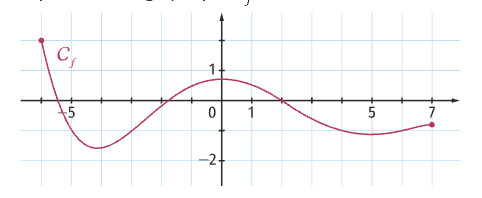
\includegraphics[scale=1.05]{ExoOblLLS23-img01}
	\end{minipage}
	
	\begin{corrBox}
		\textbf{1)} Le point de $C_f$ d'abscisse $2$ est sur l'axe des abscisses : $\mRouge{f(2)=0}$.
	\end{corrBox}
	
	\begin{corrBox}
		\textbf{2)} On cherche les abscisses des points d'intersection de $C_f$ avec la droite d'équation $y=-1$.
		
		Avec la précision permise par le graphique : $\mRouge{S\approx\{-4{,}8\ ;\ -3\ ;\ 4{,}2\ ;\ 5{,}8\}}$.
	\end{corrBox}
	
	\begin{corrBox}
		\textbf{3)} La courbe $C_f$ coupe l'axe des abscisses en 3 points (abscisses environ $-5{,}2$ ; $-1{,}2$ et $2$).
		
		L'équation $f(x)=0$ admet donc $\mRouge{3}$ \textbf{solutions} sur $[-6;7]$.
	\end{corrBox}
	
	\newpage
	%=====================================================
	\exercice{$-$ Exercice 27 p 50 $-$ Le Livre scolaire }
	
	On considère une fonction $f$ définie sur $[-4 ; 5]$ dont la représentation graphique $C_f$ est donnée ci-dessous.
	\begin{minipage}[c]{0.62\linewidth}
		\begin{enumMet}
			\item Déterminer $f(-2), f(3)$ et $f(5)$.
			\item Résoudre graphiquement l'équation $f(x)=-2$ sur $[-4 ; 5]$ ?
			\item Résoudre graphiquement l'équation $f(x)=-1$ sur $[-4;5]$?
			\item Résoudre graphiquement l'inéquation $f(x)>-2$ sur $[-4 ; 5]$.
			\item Donner un nombre réel $a$ admettant un unique antécédent par $f$.
		\end{enumMet}
	\end{minipage} \hfill
	\begin{minipage}[c]{0.38\linewidth}
		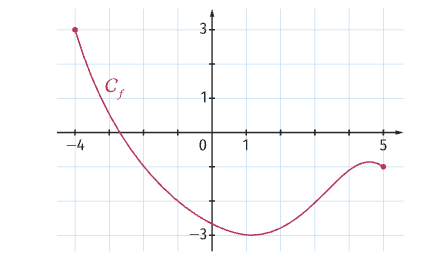
\includegraphics[scale=1.05]{ExoOblLLS27-img02}
	\end{minipage}
	
	\begin{corrBox}
		\textbf{1)} Par lecture graphique : $\mRouge{f(-2)=-1}$ \quad ; \quad $\mRouge{f(3)=-2}$ \quad ; \quad $\mRouge{f(5)=-1}$.
	\end{corrBox}
	
	\begin{corrBox}
		\textbf{2)} On cherche les abscisses des points de $C_f$ d'ordonnée $-2$ :
		
		$\mRouge{S=\{-1\ ;\ 3\}}$
	\end{corrBox}
	
	\begin{corrBox}
		\textbf{3)} On cherche les abscisses des points de $C_f$ d'ordonnée $-1$ :
		
		$\mRouge{S\approx\{-2\ ;\ 4\ ;\ 5\}}$
	\end{corrBox}
	
	\begin{corrBox}
		\textbf{4)} On cherche les abscisses des points de $C_f$ situés strictement au-dessus de la droite d'équation $y=-2$ :
		
		$\mRouge{S=\left[-4\,;\,-1\right[\ \cup\ \left]3\,;\,5\right]}$
	\end{corrBox}
	
	\begin{corrBox}
		\textbf{5)} Par exemple, $\mRouge{a=2}$ : la droite d'équation $y=2$ ne coupe $C_f$ qu'en un seul point (sur la partie gauche de la courbe).
		
		\emph{Autres réponses possibles : $a=3$ (antécédent $-4$) ou $a=-3$ (antécédent $1$, le minimum de $f$).}
	\end{corrBox}
	
	%=====================================================
	\exercice{$-$ Exercice 28 p 50 $-$ Le Livre scolaire }
	
	On considère la fonction $g$ dont la représentation graphique $\mathcal{C}_g$ est donnée ci-dessous.
	
	\begin{minipage}[c]{0.62\linewidth}
		\begin{enumMet}
			\item Résoudre l'équation $g(x)=1 \operatorname{sur}[-4 ; 5]$.
			\item Déterminer graphiquement $g(5)$.
			\item Résoudre l'inéquation $g(x)<-2$ sur [-4; 5].
			\item Donner un réel qui possède exactement quatre antécédents par la fonction $g$.
		\end{enumMet}
	\end{minipage} \hfill
	\begin{minipage}[c]{0.38\linewidth}
		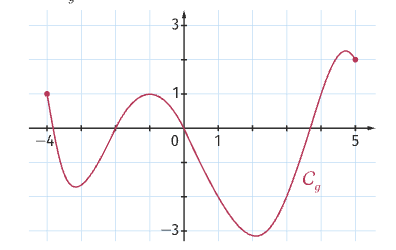
\includegraphics[scale=1.05]{ExoOblLLS28-img03}
	\end{minipage}
	
	\begin{corrBox}
		\textbf{1)} On cherche les abscisses des points de $\mathcal{C}_g$ d'ordonnée $1$ :
		
		$\mRouge{S\approx\{-4\ ;\ -1\ ;\ 4\}}$
	\end{corrBox}
	
	\begin{corrBox}
		\textbf{2)} Le point de $\mathcal{C}_g$ d'abscisse $5$ a pour ordonnée $2$ : $\mRouge{g(5)=2}$.
	\end{corrBox}
	
	\begin{corrBox}
		\textbf{3)} On cherche les abscisses des points de $\mathcal{C}_g$ situés strictement en dessous de la droite d'équation $y=-2$ :
		
		$\mRouge{S\approx\left]1{,}2\,;\,2{,}8\right[}$
	\end{corrBox}
	
	\begin{corrBox}
		\textbf{4)} Par exemple $\mRouge{0}$ : la droite d'équation $y=0$ (l'axe des abscisses) coupe $\mathcal{C}_g$ en exactement 4 points. $0$ possède donc exactement quatre antécédents par $g$.
		
		\emph{Tout réel strictement compris entre le minimum local de gauche (environ $-1{,}5$) et $1$ convient.}
	\end{corrBox}
	
	%=====================================================
	\exercice{$-$ Exercice 52 p 52 $-$ Le Livre scolaire }
	
	On considère une fonction $f$ dont la courbe représentative $C_f$ est donnée dans le repère orthonormé ci-dessous.
	
	\begin{minipage}[c]{0.55\linewidth}
		\begin{enumMet}
			\item Donner l'ensemble de définition de $f$.
			\item Résoudre graphiquement les équations et inéquations suivantes.
			\begin{multicols}{3}
				\begin{enumMet}
					\item $f(x)=-2$
					\item $f(x)=-1$
					\item $f(x)<-2$
					\item $f(x)=1$
					\item $f(x) \geqslant-2$
				\end{enumMet}
			\end{multicols}
		\end{enumMet}
	\end{minipage} \hfill
	\begin{minipage}[c]{0.48\linewidth}
		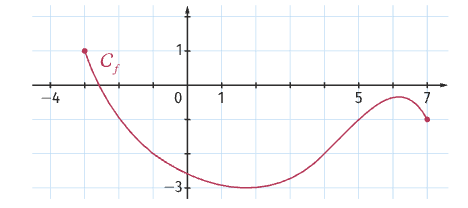
\includegraphics[scale=1.05]{ExoOblLLS52-img04}
	\end{minipage}
	
	\begin{corrBox}
		\textbf{1)} La courbe est tracée pour des abscisses allant de $-3$ à $7$ : $\mRouge{\mathcal{D}_f=[-3\,;\,7]}$.
	\end{corrBox}
	
	\begin{corrBox}
		\textbf{2) a)} $f(x)=-2$ : $\mRouge{S\approx\{-1\ ;\ 4\}}$
	\end{corrBox}
	
	\begin{corrBox}
		\textbf{2) b)} $f(x)=-1$ : $\mRouge{S\approx\{-2\ ;\ 5\ ;\ 7\}}$
	\end{corrBox}
	
	\begin{corrBox}
		\textbf{2) c)} $f(x)<-2$ : $\mRouge{S\approx\left]-1\,;\,4\right[}$
	\end{corrBox}
	
	\begin{corrBox}
		\textbf{2) d)} $f(x)=1$ : $\mRouge{S=\{-3\}}$
	\end{corrBox}
	
	\begin{corrBox}
		\textbf{2) e)} $f(x)\geqslant-2$ : $\mRouge{S\approx\left[-3\,;\,-1\right]\cup\left[4\,;\,7\right]}$
	\end{corrBox}
	
	%=====================================================
	\exercice{ $-$ Exercice 31 p 62 $-$ Parkour + $-$ Hachette technique}
	
	Soit la fonction $f$ définie sur $\mathbb{R}$ par $f(x)=3 x-1$.
	\begin{enumMet}
		\item Calculer le taux de variation de $f$ entre 1 et 2 .
		\begin{corrBox}
			$f(1)=3\times1-1=2$ et $f(2)=3\times2-1=5$.
			\[\dfrac{f(2)-f(1)}{2-1}=\dfrac{5-2}{1}=\mRouge{3}\]
		\end{corrBox}
		
		\item Calculer le taux de variation de $f$ entre 5 et 8.
		\begin{corrBox}
			$f(5)=3\times5-1=14$ et $f(8)=3\times8-1=23$.
			\[\dfrac{f(8)-f(5)}{8-5}=\dfrac{23-14}{3}=\dfrac{9}{3}=\mRouge{3}\]
		\end{corrBox}
		
		\item Que remarque-t-on ?
		\begin{corrBox}
			Les deux taux de variation sont égaux à $3$, qui est le coefficient directeur de la fonction affine $f$.
			
			Pour une fonction affine $x\mapsto mx+p$, le taux de variation est toujours égal à $m$.
		\end{corrBox}
	\end{enumMet}
	
	%=====================================================
	\exercice{ $-$ Exercice 32 p 62 $-$ Parkour + $-$ Hachette technique}
	
	Soit $f$ la fonction définie sur $\mathbb{R}$ par $f(x)=x^2$.
	\begin{enumMet}
		\item Calculer le taux de variation de $f$ entre 2 et 3.
		\begin{corrBox}
			\[\dfrac{f(3)-f(2)}{3-2}=\dfrac{9-4}{1}=\mRouge{5}\]
		\end{corrBox}
		
		\item Calculer le taux de variation de $f$ entre -3 et -1
		\begin{corrBox}
			\[\dfrac{f(-1)-f(-3)}{-1-(-3)}=\dfrac{1-9}{2}=\dfrac{-8}{2}=\mRouge{-4}\]
		\end{corrBox}
	\end{enumMet}
	
	%=====================================================
	\exercice{ $-$ Exercice 33 p 62 $-$ Parkour + $-$ Hachette technique}
	
	Soit $f$ une fonction définie par sa représentation graphique dans un repère.
	
	Avec la précision permise par le graphique :
	
	\begin{enumMet}
		\item Déterminer le taux de variation de $f$ entre -3 et -1.
		\begin{corrBox}
			Par lecture graphique : $f(-3)=0$ et $f(-1)=3$.
			\[\dfrac{f(-1)-f(-3)}{-1-(-3)}=\dfrac{3-0}{2}=\mRouge{1{,}5}\]
		\end{corrBox}
		
		\item Déterminer le taux de variation de $f$ entre 0 et 2 .
		\begin{corrBox}
			Par lecture graphique : $f(0)\approx2{,}4$ et $f(2)=0$.
			\[\dfrac{f(2)-f(0)}{2-0}\approx\dfrac{0-2{,}4}{2}\approx\mRouge{-1{,}2}\]
		\end{corrBox}
	\end{enumMet}
	
	\begin{center}
		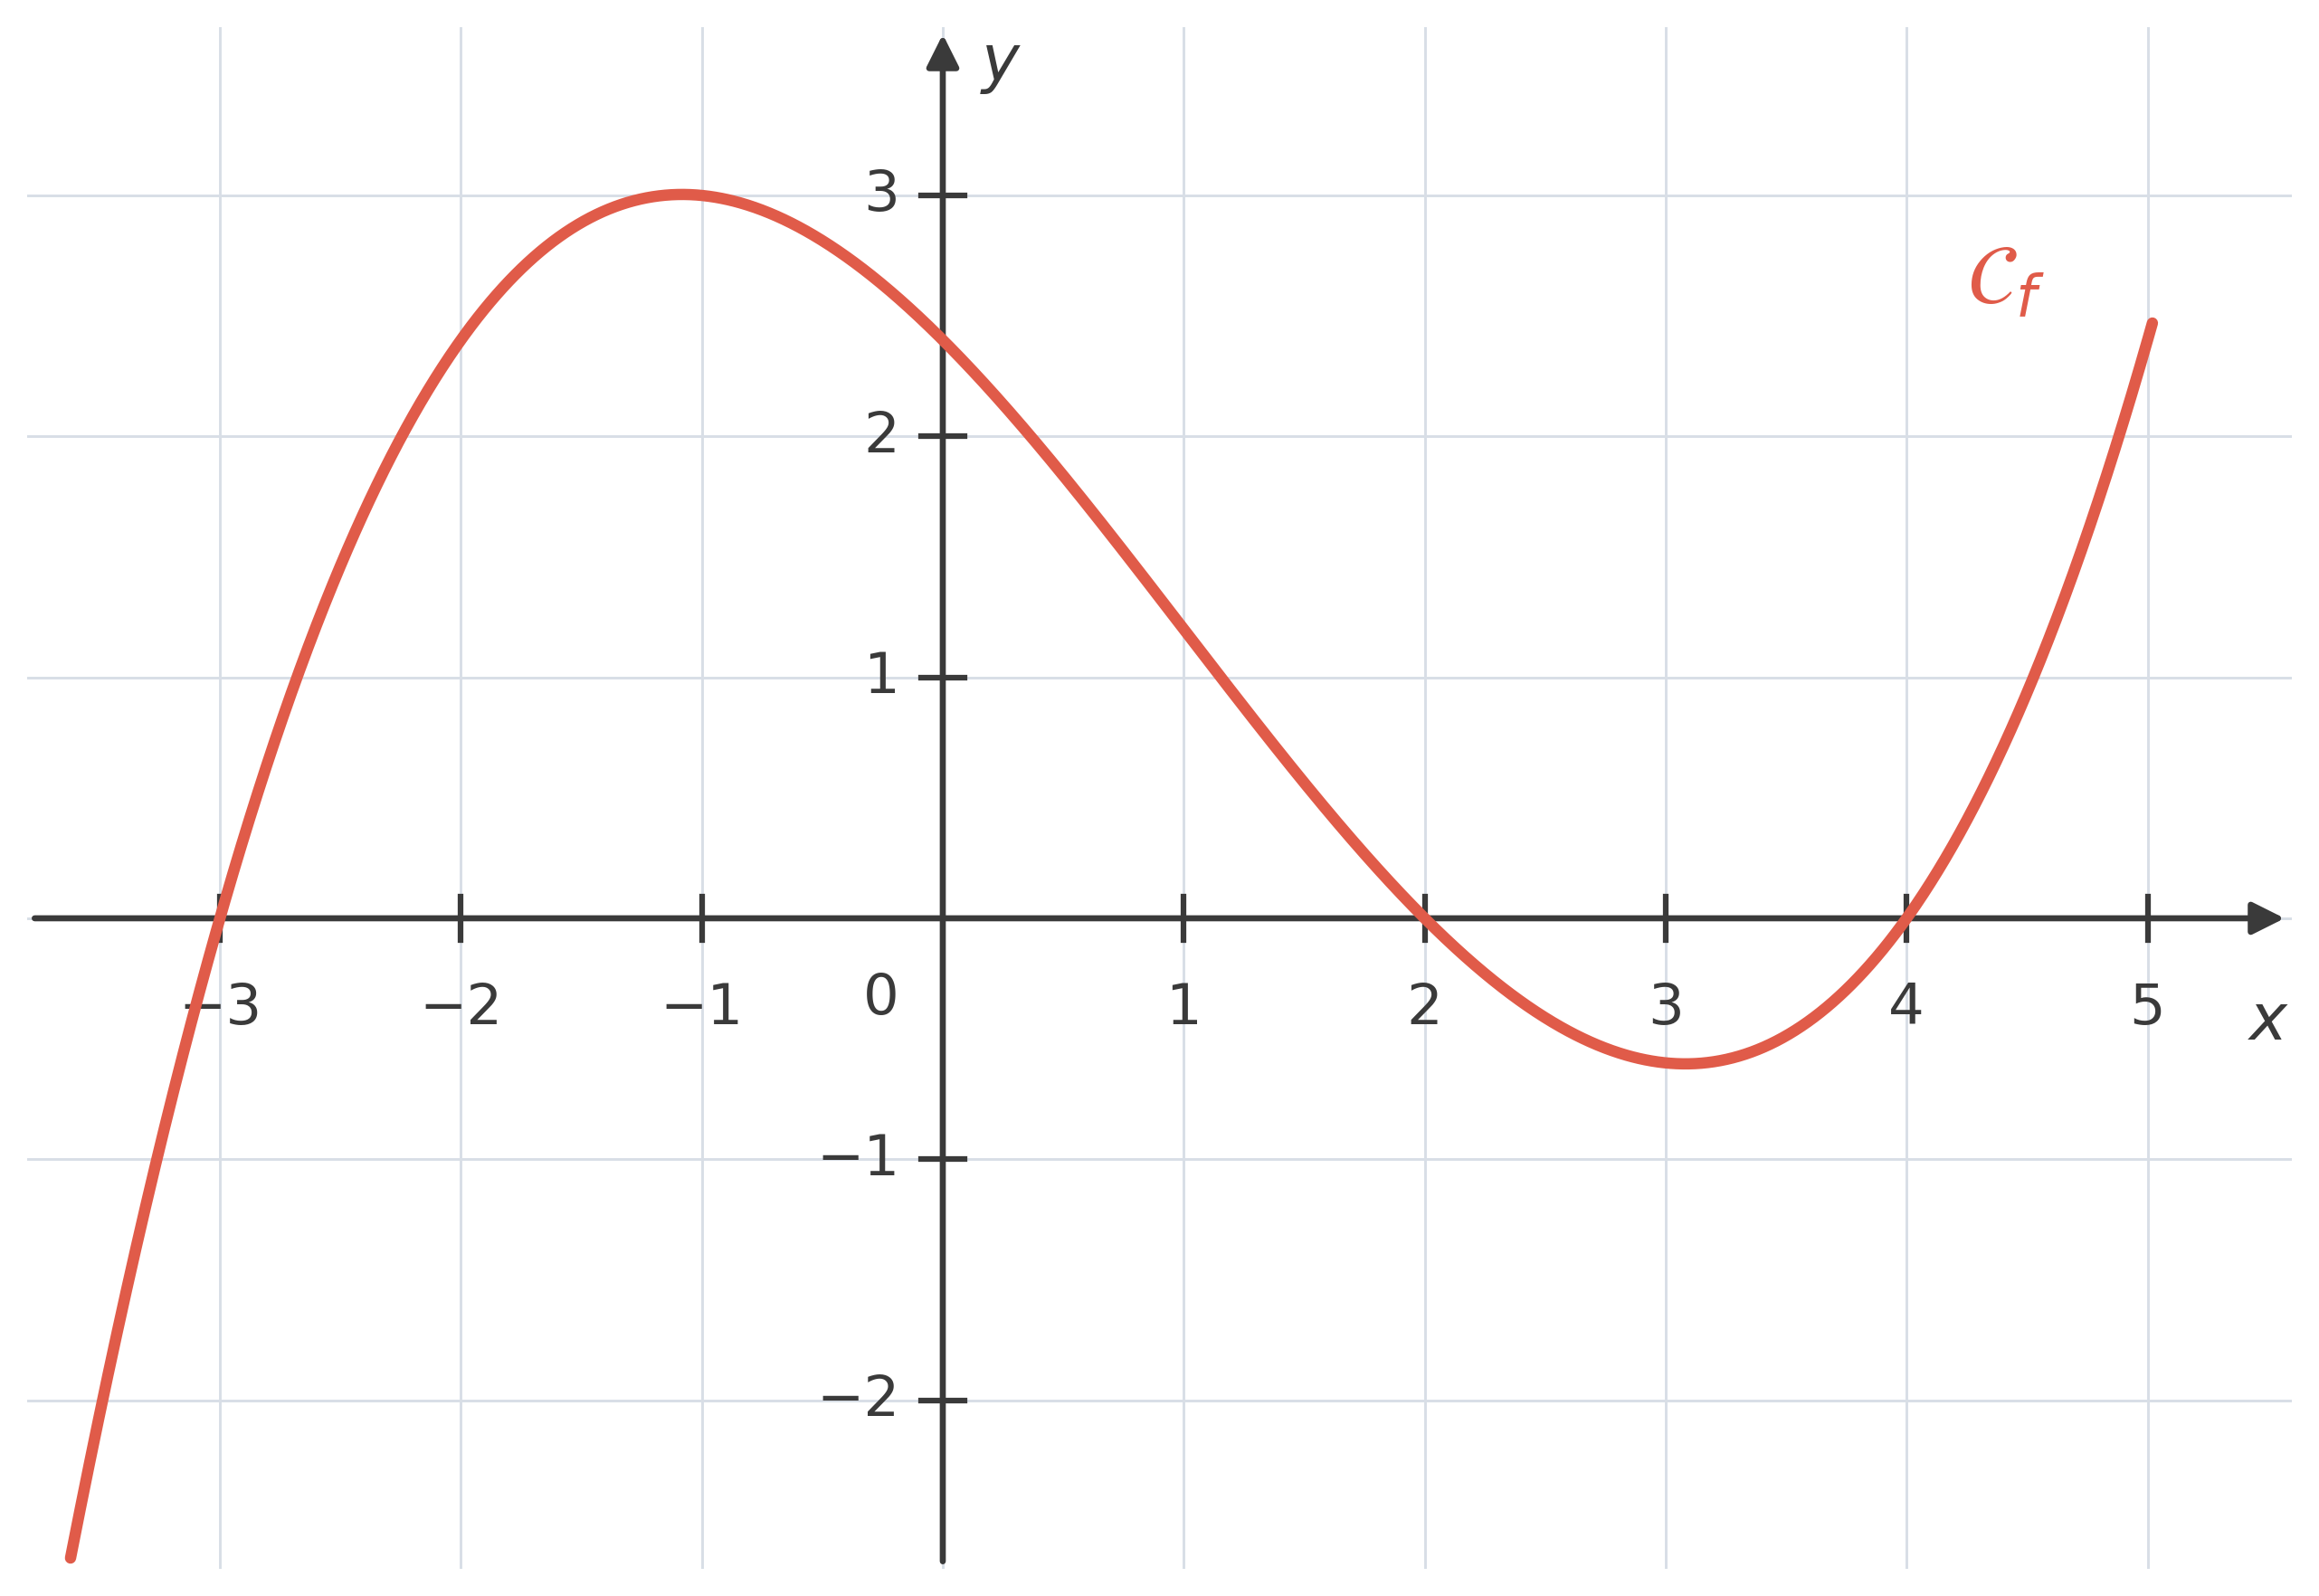
\includegraphics[scale=0.4]{ExoOblParkour+33-img06}
	\end{center}
	
	%=====================================================
	\exercice{ $-$ Exercice 34 p 62 $-$ Parkour + $-$ Hachette technique}
	
	Soit la fonction $f$ définie sur $\mathbb{R}$ par $f(x)=4 x+3$ et deux réels $x_1$ et $x_2$.
	\begin{enumMet}
		\item Calculer le taux de variation de $f$ entre $x_1$ et $x_2$. Simplifier au maximum l'expression.
		\begin{corrBox}
			Pour $x_1\neq x_2$ :
			\[\dfrac{f(x_2)-f(x_1)}{x_2-x_1}=\dfrac{(4x_2+3)-(4x_1+3)}{x_2-x_1}=\dfrac{4x_2+3-4x_1-3}{x_2-x_1}=\dfrac{4(x_2-x_1)}{x_2-x_1}=\mRouge{4}\]
		\end{corrBox}
		
		\item En déduire les variations de $f$ sur $\mathbb{R}$. 
		\begin{corrBox}
			Le taux de variation de $f$ entre deux réels quelconques est égal à $4$, qui est toujours positif.
			
			Donc $f$ est \textbf{croissante sur $\bm{\mathbb{R}}$}.
		\end{corrBox}
	\end{enumMet}
	
	%=====================================================
	\exercice{ $-$ Exercice 35 p 62 $-$ Parkour + $-$ Hachette technique}
	
	Soit la fonction $f$ définie sur $\mathbb{R}$ par $f(x)=x^2$.
	\begin{enumMet}
		\item Calculer le taux de variation de $f$ entre 1 et 2 .
		\begin{corrBox}
			\[\dfrac{f(2)-f(1)}{2-1}=\dfrac{4-1}{1}=\mRouge{3}\]
		\end{corrBox}
		
		\item On considère deux réels $x_1$ et $x_2$. Calculer le taux de variation de $f$ entre $x_1$ et $x_2$. Simplifier au maximum l'expression.
		\begin{corrBox}
			Pour $x_1\neq x_2$, en utilisant l'identité remarquable $a^2-b^2=(a-b)(a+b)$ :
			\[\dfrac{f(x_2)-f(x_1)}{x_2-x_1}=\dfrac{x_2^2-x_1^2}{x_2-x_1}=\dfrac{(x_2-x_1)(x_2+x_1)}{x_2-x_1}=\mRouge{x_1+x_2}\]
		\end{corrBox}
		
		\item Donner le signe du taux de variation dans le cas où $x_1$ et $x_2$ sont positifs, puis dans le cas où $x_1$ et $x_2$ sont négatifs.
		\begin{corrBox}
			Si $x_1$ et $x_2$ sont positifs (et distincts), leur somme $x_1+x_2$ est \textbf{positive}.
			
			Si $x_1$ et $x_2$ sont négatifs (et distincts), leur somme $x_1+x_2$ est \textbf{négative}.
		\end{corrBox}
		
		\item En déduire les variations de $f$ sur $\mathbb{R}$.
		\begin{corrBox}
			La fonction $f$ est \textbf{décroissante sur $\bm{]-\infty\,;\,0]}$} et \textbf{croissante sur $\bm{[0\,;\,+\infty[}$}.
		\end{corrBox}
	\end{enumMet}
	
	%=====================================================
	\exercice{ $-$ Exercice 37 p 62 $-$ Parkour + $-$ Hachette technique}
	
	On donne dans un repère la courbe représentative de la fonction $f$ et deux points A et B.
	\begin{center}
		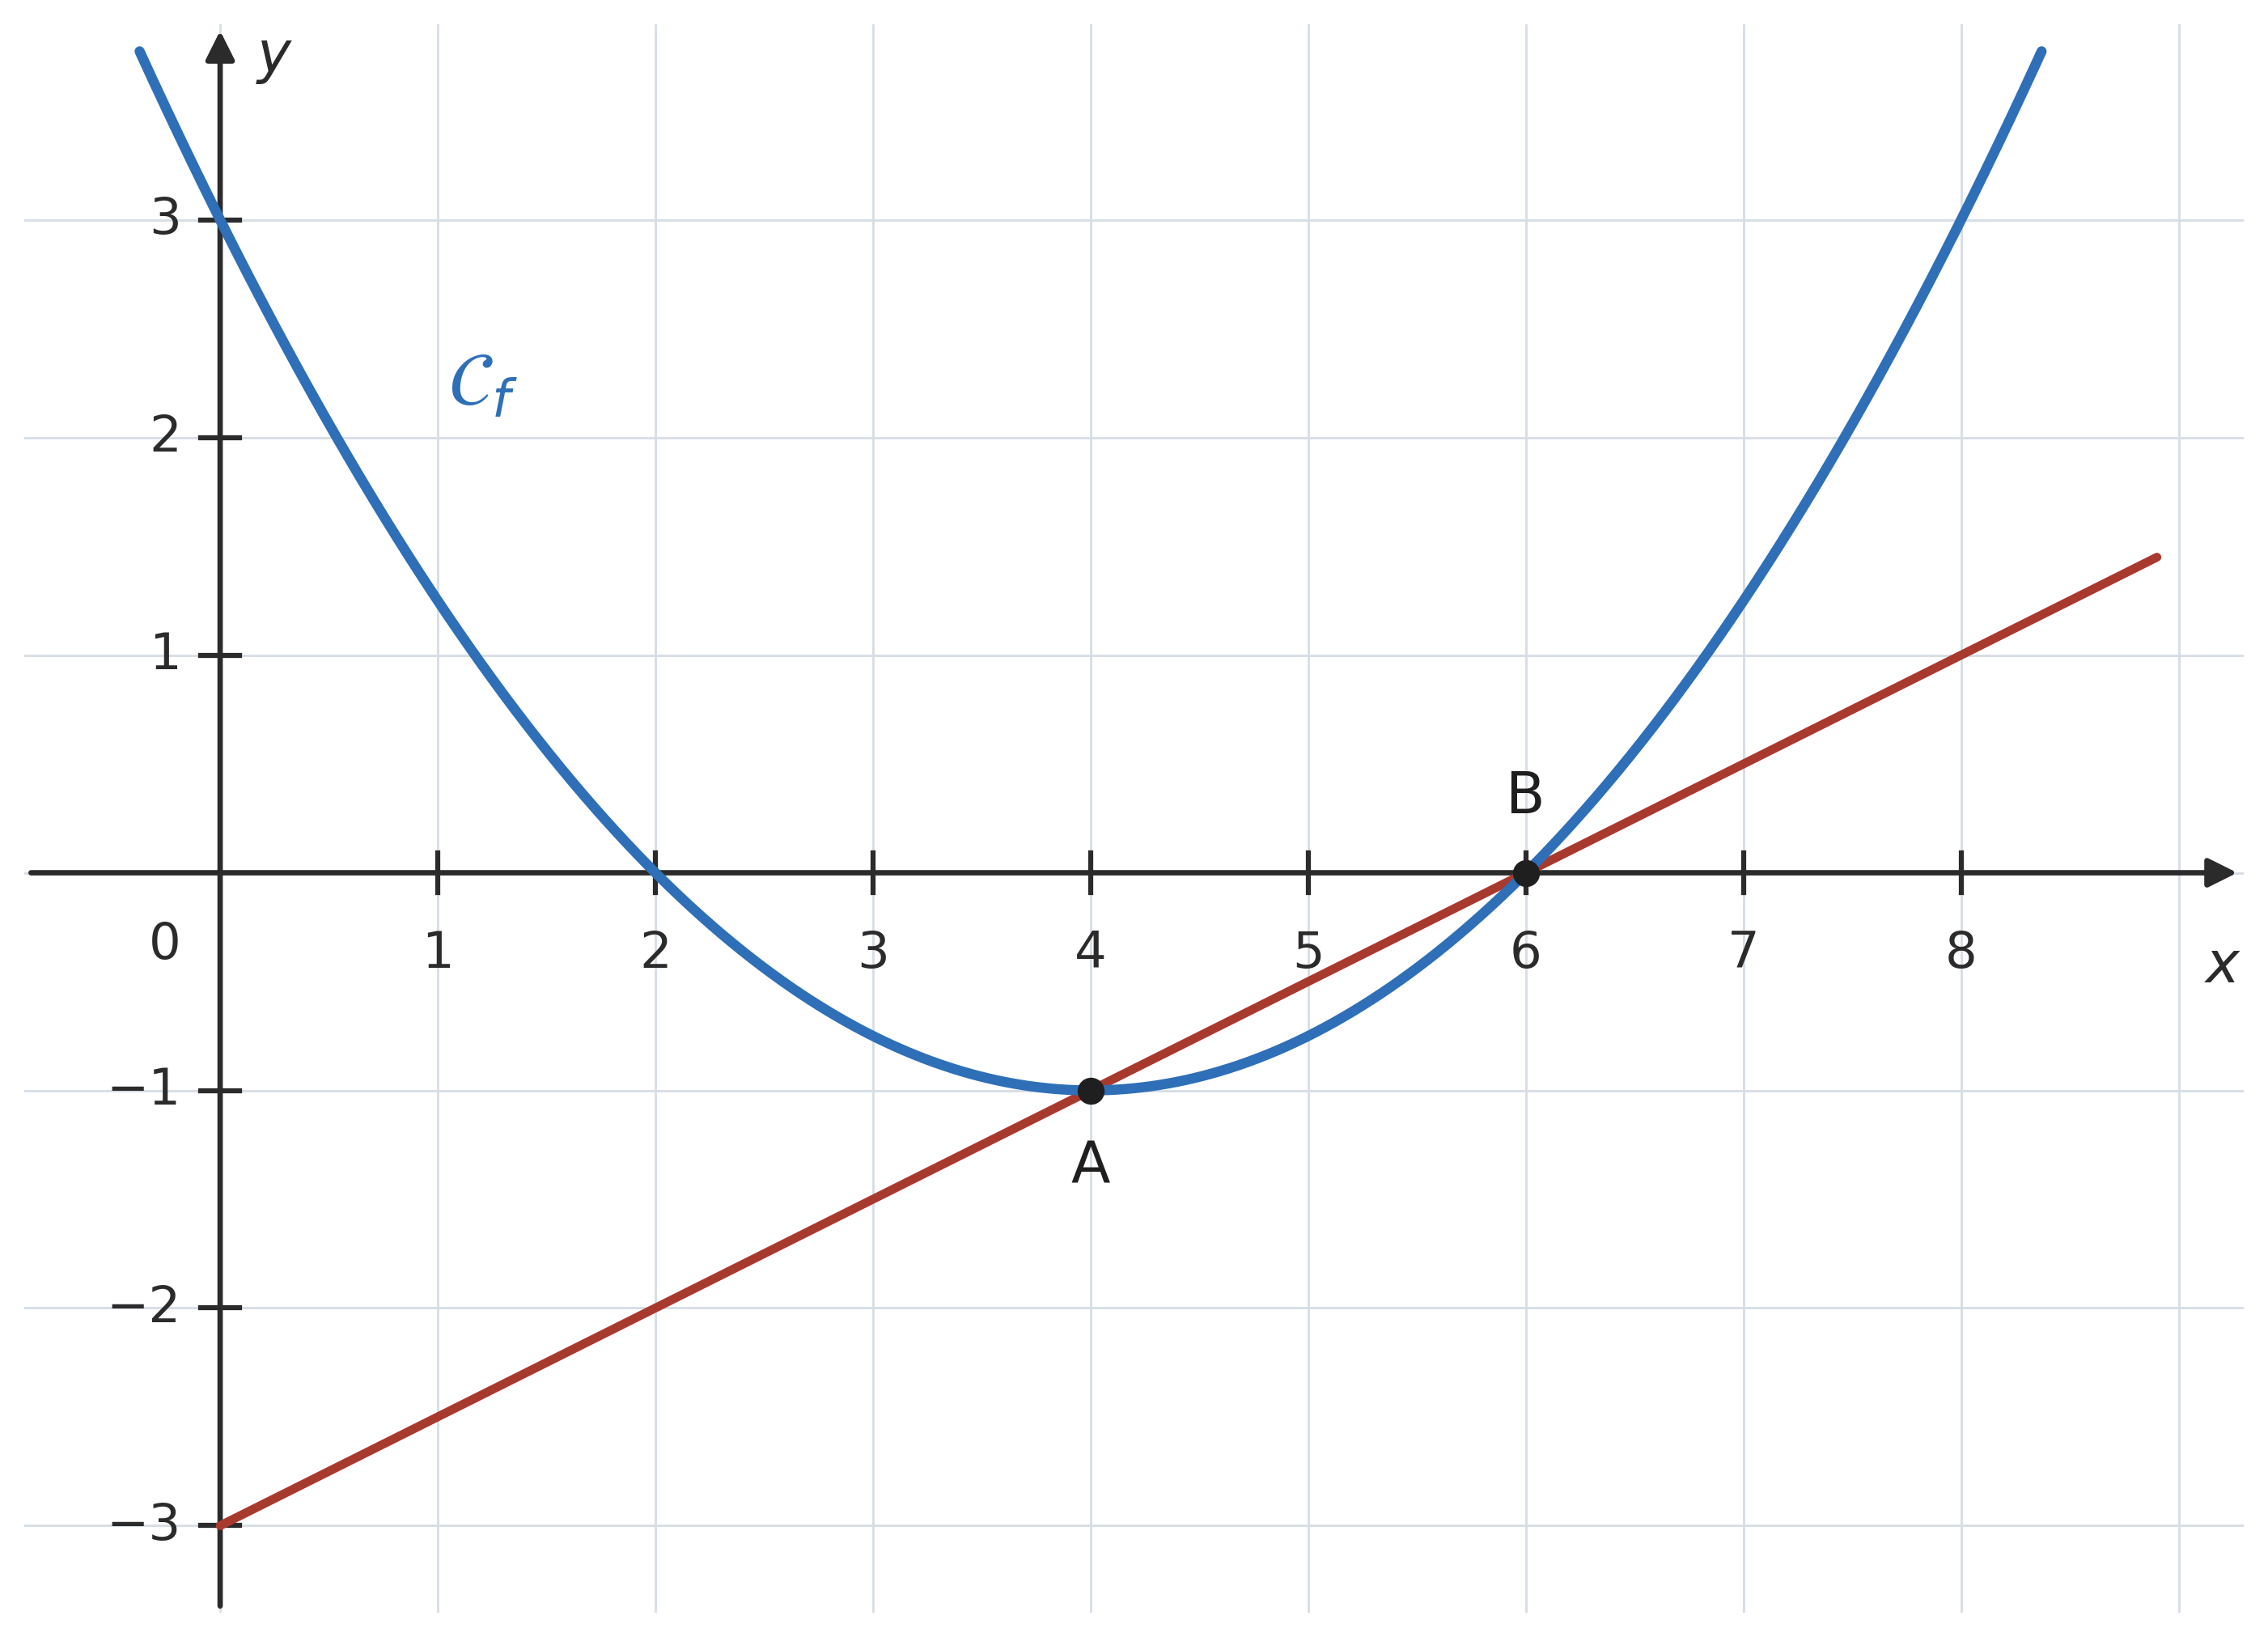
\includegraphics[scale=0.4]{ExoOblParkour+37-img07}
	\end{center}
	\begin{enumMet}
		\item Lire les coordonnées de A et B sur le graphique et en déduire le coefficient directeur de la droite (AB).
		\begin{corrBox}
			On lit $A(4\,;\,-1)$ et $B(6\,;\,0)$.
			\[m=\dfrac{y_B-y_A}{x_B-x_A}=\dfrac{0-(-1)}{6-4}=\mRouge{\dfrac{1}{2}}\]
		\end{corrBox}
		
		\item On admet que la fonction a pour expression :$f(x)=\dfrac{1}{4}(x-2)(x-6)$
		
		Déterminer le taux de variation de $f$ entre 4 et 6 .
		\begin{corrBox}
			$f(4)=\dfrac{1}{4}\times(4-2)\times(4-6)=\dfrac{1}{4}\times2\times(-2)=-1$ \quad et \quad $f(6)=\dfrac{1}{4}\times4\times0=0$.
			\[\dfrac{f(6)-f(4)}{6-4}=\dfrac{0-(-1)}{2}=\mRouge{\dfrac{1}{2}}\]
		\end{corrBox}
		
		\item Quel lien existe-t-il entre les résultats précédents?
		\begin{corrBox}
			Les deux résultats sont égaux : le taux de variation de $f$ entre $4$ et $6$ est égal au coefficient directeur de la sécante $(AB)$, où $A$ et $B$ sont les points de $C_f$ d'abscisses $4$ et $6$.
		\end{corrBox}
	\end{enumMet}
	
	\newpage
	
	%=====================================================
	\exercice{ $-$ Exercice 9 p 55 $-$ Calao}
	
	On considère la fonction $x \mapsto \dfrac{1}{x}$, et deux réels $x_1$ et $x_2$ distincts non nuls.
	\begin{enumMet}
		\item Exprimer le taux de variation entre $x_1$ et $x_2$.
		\begin{corrBox}
			\[\dfrac{f(x_2)-f(x_1)}{x_2-x_1}=\dfrac{\dfrac{1}{x_2}-\dfrac{1}{x_1}}{x_2-x_1}\]
		\end{corrBox}
		
		\item Simplifier au mieux le quotient.
		\begin{corrBox}
			On réduit le numérateur au même dénominateur : $\dfrac{1}{x_2}-\dfrac{1}{x_1}=\dfrac{x_1-x_2}{x_1x_2}=\dfrac{-(x_2-x_1)}{x_1x_2}$.
			
			D'où :
			\[\dfrac{f(x_2)-f(x_1)}{x_2-x_1}=\dfrac{-(x_2-x_1)}{x_1x_2}\times\dfrac{1}{x_2-x_1}=\mRouge{-\dfrac{1}{x_1x_2}}\]
		\end{corrBox}
		
		\item Étudier son signe suivant le signe de $x_1$ et $x_2$.
		\begin{corrBox}
			\textbf{Si $\bm{x_1}$ et $\bm{x_2}$ sont de même signe} (tous deux strictement positifs ou tous deux strictement négatifs) : $x_1x_2>0$, donc $-\dfrac{1}{x_1x_2}<0$. Le taux de variation est \textbf{négatif}.
			
			\textbf{Si $\bm{x_1}$ et $\bm{x_2}$ sont de signes contraires} : $x_1x_2<0$, donc $-\dfrac{1}{x_1x_2}>0$. Le taux de variation est \textbf{positif}.
		\end{corrBox}
		
		\item En déduire la monotonie de la fonction inverse, en précisant l'intervalle.
		\begin{corrBox}
			Sur chacun des intervalles $]-\infty\,;\,0[$ et $]0\,;\,+\infty[$, deux réels $x_1$ et $x_2$ sont de même signe, donc le taux de variation est négatif.
			
			La fonction inverse est \textbf{strictement décroissante sur $\bm{]-\infty\,;\,0[}$} et \textbf{strictement décroissante sur $\bm{]0\,;\,+\infty[}$}.
			
			\emph{Attention : elle n'est pas décroissante sur $\mathbb{R}^*$ tout entier, car par exemple $-1<1$ et $f(-1)=-1<f(1)=1$.}
		\end{corrBox}
	\end{enumMet}
	
	%=====================================================
	\exercice{ $-$ Exercice 10 p 55 $-$ Calao}
	
	Soit $f$ définie sur $]-2 ;+\infty\left[\right.$ par $f(x)=\dfrac{-4}{x+2}$ et deux réels distincts $x_1$ et $x_2$ de $]-2 ;+\infty[$.
	\begin{enumMet}
		\item Exprimer le taux de variation entre $x_1$ et $x_2$.
		\begin{corrBox}
			On calcule d'abord la différence des images :
			\[f(x_2)-f(x_1)=\dfrac{-4}{x_2+2}+\dfrac{4}{x_1+2}=\dfrac{-4(x_1+2)+4(x_2+2)}{(x_1+2)(x_2+2)}=\dfrac{4x_2-4x_1}{(x_1+2)(x_2+2)}=\dfrac{4(x_2-x_1)}{(x_1+2)(x_2+2)}\]
			D'où :
			\[\dfrac{f(x_2)-f(x_1)}{x_2-x_1}=\mRouge{\dfrac{4}{(x_1+2)(x_2+2)}}\]
		\end{corrBox}
		
		\item Conclure sur la monotonie de la fonction $f$.
		\begin{corrBox}
			Comme $x_1>-2$ et $x_2>-2$, on a $x_1+2>0$ et $x_2+2>0$, donc $(x_1+2)(x_2+2)>0$.
			
			Le taux de variation $\dfrac{4}{(x_1+2)(x_2+2)}$ est donc strictement positif.
			
			La fonction $f$ est \textbf{strictement croissante sur $\bm{]-2\,;\,+\infty[}$}.
		\end{corrBox}
	\end{enumMet}
	
	%=====================================================
	\exercice{ $-$ Exercice 11 p 55 $-$ Calao}	
	
	On considère la fonction $f$ représentée par la courbe C.
	\begin{center}
		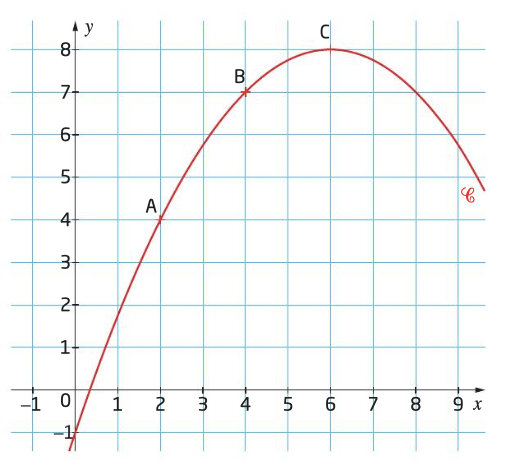
\includegraphics[scale=0.8]{ExoOblCalao11-img08}
	\end{center}
	\begin{enumMet}
		\item \begin{enumMet}
			\item Lire la pente des sécantes (AB) et (BC).
			\begin{corrBox}
				On lit $A(2\,;\,4)$, $B(4\,;\,7)$ et $C(6\,;\,8)$.
				
				Pente de $(AB)$ : $m_{AB}=\dfrac{7-4}{4-2}=\mRouge{\dfrac{3}{2}}=1{,}5$
				
				Pente de $(BC)$ : $m_{BC}=\dfrac{8-7}{6-4}=\mRouge{\dfrac{1}{2}}=0{,}5$
			\end{corrBox}
			
			\item Déterminer leur équation réduite.
			\begin{corrBox}
				\textbf{Droite $\bm{(AB)}$ :} $y=1{,}5x+p$. Elle passe par $A(2\,;\,4)$ : $4=1{,}5\times2+p$, donc $p=1$.
				
				$\mRouge{(AB) : y=1{,}5x+1}$
				
				\textbf{Droite $\bm{(BC)}$ :} $y=0{,}5x+p$. Elle passe par $B(4\,;\,7)$ : $7=0{,}5\times4+p$, donc $p=5$.
				
				$\mRouge{(BC) : y=0{,}5x+5}$
			\end{corrBox}
		\end{enumMet}
		
		\item La courbe C a pour équation $y=\dfrac{-x^2}{4}+3 x-1$.
		\begin{enumMet}
			\item Calculer le taux de variation de $f$ entre 0 et 2 .
			\begin{corrBox}
				$f(0)=0+0-1=-1$ \quad et \quad $f(2)=\dfrac{-4}{4}+6-1=-1+6-1=4$.
				\[\dfrac{f(2)-f(0)}{2-0}=\dfrac{4-(-1)}{2}=\mRouge{\dfrac{5}{2}}=2{,}5\]
			\end{corrBox}
			
			\item Calculer le taux de variation de $f$ entre 3,9 et 4 . On utilisera au mieux la calculatrice.
			\begin{corrBox}
				$f(3{,}9)=\dfrac{-3{,}9^2}{4}+3\times3{,}9-1=\dfrac{-15{,}21}{4}+11{,}7-1=-3{,}8025+10{,}7=6{,}8975$
				
				$f(4)=\dfrac{-16}{4}+12-1=-4+12-1=7$
				\[\dfrac{f(4)-f(3{,}9)}{4-3{,}9}=\dfrac{7-6{,}8975}{0{,}1}=\dfrac{0{,}1025}{0{,}1}=\mRouge{1{,}025}\]
			\end{corrBox}
		\end{enumMet}
	\end{enumMet}
	
\end{document}